\fancyhead[LO]{{\scriptsize {\FA \ }我们最幸福 {\FA } 神的黄昏}}%奇數頁眉的左邊
\fancyhead[RO]{{\tiny{\textcolor{Gray}{\FA \ }}}\thepage}
\fancyhead[LE]{{\tiny{\textcolor{Gray}{\FA \ }}}\thepage}
\fancyhead[RE]{{\scriptsize {\FA \ }我们最幸福 {\FA } 神的黄昏}}%偶數頁眉的右邊
\fancyfoot[LE,RO]{}
\fancyfoot[LO,CE]{}
\fancyfoot[CO,RE]{}
\chapter*{06 {\FA } 神的黄昏}
\addcontentsline{toc}{chapter}{\hspace{5mm}06 \textbf{>}\ \ 神的黄昏}
\vspace{5mm}
\begin{flushright}
	\textcolor{PinYinColor}{\EN \huge{Twilight\\
		of the God\\
	\ \\}}
\end{flushright}

\begin{figure}[!htbp]
	\centering
	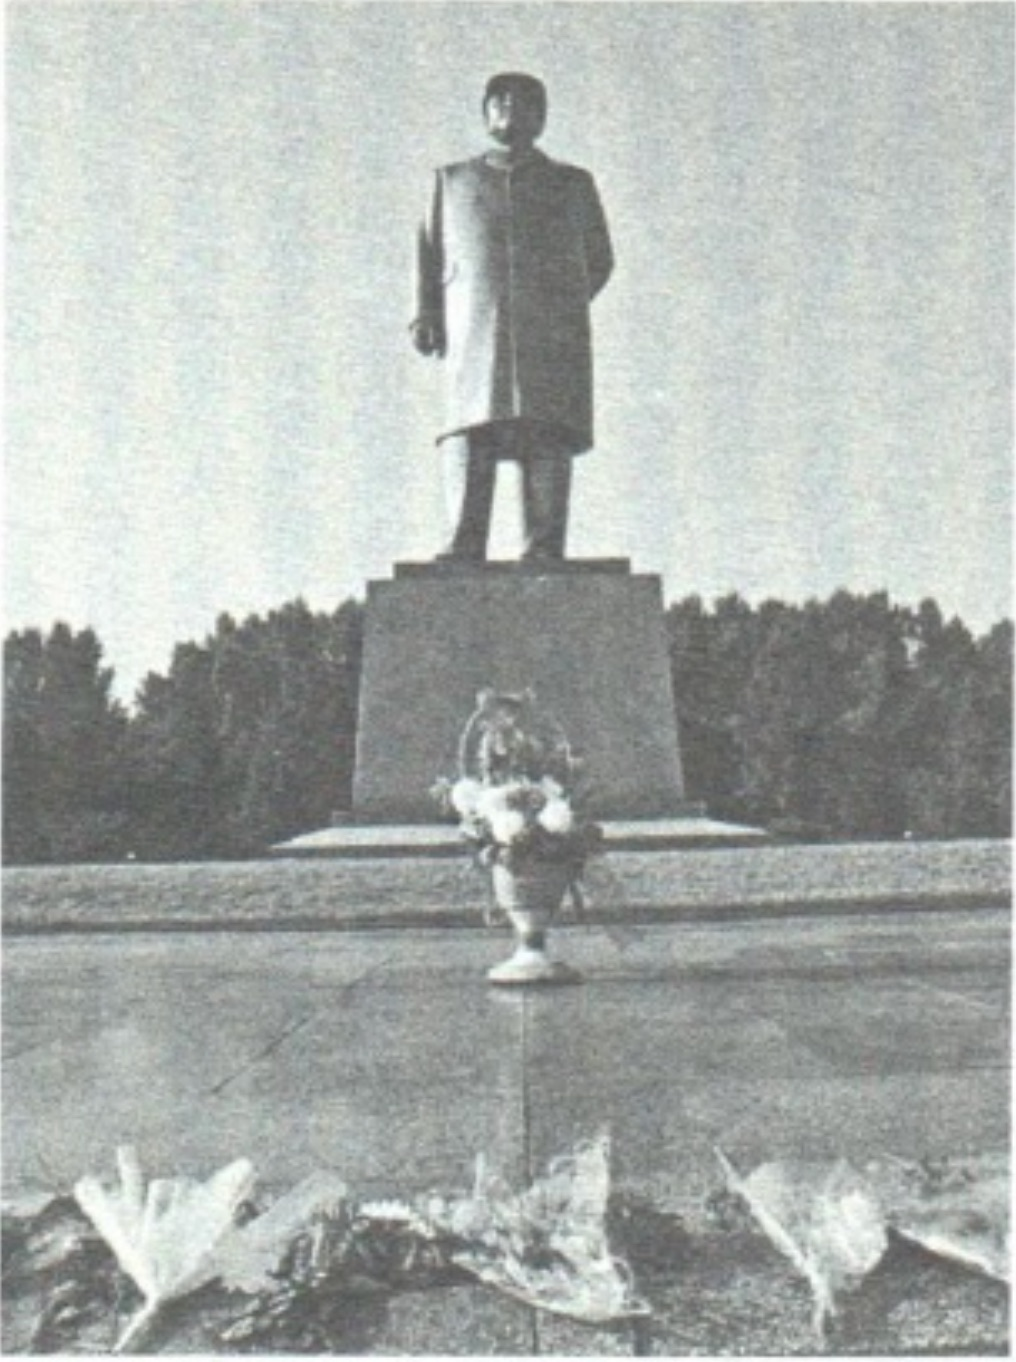
\includegraphics[width=6cm]{./Chapters/Images/06.jpg}
	\caption*{清津的金日成雕像}
\end{figure}

\ifnum\theparacolNo=2
	\begin{multicols}{\theparacolNo}
\fi
在1994年7月,美兰只剩一门考试,之后就可以从师范学院毕业。那时她作为见习教师被分配到清津市内的一所幼儿园。在7月9号中午的时候,孩子们都回家吃午饭了。她在教师休息室里,正准备打开从家里带来的盒饭同其它老师共进午餐,这时候,突然她听见一阵急促的脚步声从走廊传过来。于是就走出了房间,一个小女孩刚刚从家里跑回来。马尾辫都给汗水打湿了、跑得上气不接下气、语无伦次的,没人听得懂她在说什么。\\

“他死了,他死了。”小女孩喊着,在喘气之间吐出这么几个字。\\

“你在说什么?”一个老师问。\\

“伟大的统帅死了!”\\

这个词只能被用于称呼金日成。老师们惊呆了,任何人即使是孩子都知道这么说。在幼儿园,孩子们从小就被教育不能拿领袖来开玩笑。他们抓住女孩的肩膀试图让她平静下来。她正大口喘着粗气。\\

“真是反党的胡言乱语。”一个老师责备道。\\

“不,不。我刚刚在家看了电视。”女孩坚持着。\\

老师们都不相信她。他们清楚5岁大的孩子还分不清事情的真假。再说了,电视新闻一般下午5点之后才会播放。然而他们也开始不安起来,因此也顾不上吃饭,想弄清楚到底发生了什么。学校没有收音机或电视机,所以他们都跑到大街上去了。那个小女孩很急切的领着他们去几个街区之外自己的家。当他们上楼的时候,发现那里挤满了人,他们不得不推搡着才能挤到电视跟前。美兰也设法挤了进去。她什么都听不见,但是她看见周围满是悲伤、苍白的脸。人群里发出一阵呜咽,转而嚎啕大哭。从开着的窗户外,可以听见经过昨夜的大雨至今仍湿漉漉的整条大街都在哀号。\\

美兰脑子里一片空白。她无法理解。她只是个实习老师,一个受高等过教育的女性,她明白人终将一死,生命是有限的。但是她想金日成可不是凡人。如果伟大统帅都会死,那么还有什么不会发生。\\

所有的北朝鲜人都异常清晰的记得,当他们得知金日成的死讯时,自己在做什么。多年来,每每采访脱北者,当我问道“那时候,你在哪里呢?”无论我采访的主题是什么,无论被采访者多么健忘,或者多么不配合,他们对这个话题总是会娓娓道来。经历了90年代梦魇般岁月的人们,依旧能够如数家珍般的立即描述出那一天他们的一举一动。在这个受到如此巨大冲击的时刻,一切时间法则,一切人类意识全部冻结了。\\

金日成死的这一年,也是自朝鲜战争以来,全世界最热闹的一年,重大事件频发。面对濒临崩溃的经济,再加上中国和俄罗斯现在同敌人在首尔打得火热,北朝鲜很快沦为流氓国家。联合国,在咄咄逼人的新任美国总统比尔克林顿(Bill Clinton)的把持下,要求北朝鲜开放其核设施接受核查。在1993年3月,为进一步发展核武器,北朝鲜宣布退出核不扩散条约,引发冷战后第一次核恐慌。第二年,北朝鲜更进一步,对宁边核反应堆的核燃料棒钚进行处理。宁边位于平壤以北65公里,是北朝鲜秘密的核武研究中心,对此,五角大楼甚至威胁实施先发制人的打击。北朝鲜则以战争相回应。正是在此时,北朝鲜的谈判者提出了日后著名的威胁“将首尔变成一片火海。”\\

在6月,美国前总统吉米·卡特(Jimmy Carter)突然对北朝鲜进行了三天的访问。期间卡特(Jimmy Carter)抛出一个提议,北朝鲜冻结其核计划,作为交换美国提供能源援助。卡特还转达了北朝鲜对时任南韩总统金泳三访问平壤的邀请。敌对多年的两国领导人计划于1994年7月25日进行此次具有划时代意义的会面。\\

7月6日,金日成前往平壤以北的一个山区别墅视察,金日成拟在此处接见南韩总统。期间,他还前往附近的一个集体农庄,进行其著名的“现场指导”。那天,天气非常炎热,气温大概35度。晚餐过后,金日成突发严重心脏病。几个小时后,他就去世了。34个小时之后,他的死讯才被公布。虽然金正日早在20年前就被定为继任者,但是平壤需要时间好好准备如何冠冕堂皇的宣布这样一个共产世界里第一例子承父业的权力继承。\\

去世时,金日成已82岁高龄,远远超过他那一代北朝鲜男性的预期寿命。那时,他颈部已经长有一个高尔夫球般大小的很明显的甲状腺瘤。因此,除了北朝鲜民众,所有人都很清楚,他其实时日无多,但是从没有任何公开的关于金健康状况恶化的讨论。他不仅仅是这个国家的父亲、他们的华盛顿、他们的毛、还是他们的神。\\

宋女士,那时正在家为自己和丈夫准备午餐。工厂已经关门了,长博也因拿不到工资,现在也很少去电台上班。他正坐在正屋里等着电视新闻开播。他们听说,正午时分会有特别新闻播报,想必应该和正在进行的核谈判有关。一个月前,当北朝鲜宣布不再同国际原子能机构合作时,也曾有过一次这样的特别新闻播报。长博作为一个记者,自然也十分关注此次的外交角力。而宋女士却对什么核武器谈判没什么兴趣。她有更多眼前的烦恼:例如怎么才能使玉米粥看上去更可口一些之类的事情。突然她听见长博打着响指。\\

“有事情发生了,大事情。”他喊道。\\

宋女士把脑袋从分割厨房和主屋的隔断上的一个小窗口探过来。她正好看到一些不对头的东西。电视新闻主持人全部穿着丧服,黑西装打着黑领带。她赶紧用毛巾擦干手,跑到客厅来看电视。\\

北朝鲜劳动党中央委员会、中央军事委员会、国防委员会、中央人民委员会、朝鲜人民民主主义人民共和国国务院以最悲痛的心情向全体国民宣告,北朝鲜劳动党中央总书记、朝鲜人民民主主义人民共和国主席、伟大领袖金日成同志,突然因病于今天凌晨2时去世。\\

我们倍受尊敬的慈父般的领袖,他为了人民群众的独立事业奉献终身,为了祖国的繁荣、人们的幸福而鞠躬尽瘁,为了统一祖国,独立自主的屹立于世界,操劳到生命的最后一刻,现在离我们而去,令我们深感悲痛。\\

宋女士脑子里一片空白。浑身像是被电流击中,好像刽子手按下电椅按钮。这种感觉她以前只有过一次,那是几年前当她得知母亲死讯的时候,但是那次,对于母亲的去世,她是有心理准备的。她从来没有听说金日成有什么病痛;仅仅3周之前,他们还在电视上看到他精力充沛的会见吉米·卡特(Jimmy Carter)。这不可能是真的。她试图集中精神好好听听电视里说什么。他的嘴唇在动着,但是却不知所云。难以置信。她开始嚎啕大哭。\\

“这让我们怎么活啊?没有统帅,我们该怎么做啊?”这些话脱口而出。\\

她丈夫根本没有反映。脸色苍白,面无表情的凝视这半空。宋女士却不能保持安静,整个身体热血翻涌。她冲下楼来到房子前面的院子。很多邻居也来了。他们双膝跪倒,以头呛地。恸哭声响彻云霄。\\

宋女士的大女儿玉熙结婚以后辞去了在建筑公司宣传部门的工作,但是她仍然时不时的被小区叫去参加义务演出。她曾经接受过播音员的专业训练,用车载扬声器鼓励工人们努力完成工作指标。她清晰且权威式的声音在哪里都有用武之地。玉熙也不可能拒绝当地公安局要求她去解说一个希望公众配合的短片。还必须非常严肃的去背诵大量诸如“让我们抓住更多的奸细来保卫祖国。”和“如果犯罪,立即坦白。”这类的话。\\

彩排之后,她精疲力尽的慢慢踱回家,期待着马上吃午饭。此时玉熙注意到大街上空空荡荡。她和丈夫还有两个孩子住在熙熙攘攘的清津火车站的斜对面。\\

当她上了楼,她很惊奇的发现门锁上了,她知道丈夫此时应该在家的。她还听见旁边公寓里传出了电视机的声音。她轻轻推开门,朝里面张望。她丈夫正和其它邻居们一起,盘着腿坐在地板上。他眼睛红红的,但是此时,他没有喝醉。\\

“嘿,怎么啦?怎么中午也放新闻?”她问道。\\

“闭嘴,自己看。”她丈夫吼道。对他易怒的脾气已经习以为常,玉熙也没多说什么。\\

房间里每个人都在哭。是的,每个人、除了玉熙。她觉得脑子里一片空白、不是悲伤、不是高兴,可能有点恼怒。她现在想到的只是饥肠辘辘的肚子,对其他的她毫无兴趣。金日成可能死了,她想,但是我还活着,我要吃东西。为了不引起注意,她尽可能静静的坐着,也不知过了多久,她起身离开。\\

“好了,我要回家准备中饭了。”她告诉丈夫。\\

他非常鄙夷的看了她一眼。虽然因为酗酒和坏脾气使得他没有机会加入劳动党,永洙却自视是个高级干部,喜欢以自己的标准对周围的人指手划脚。在家,因为玉熙拒绝做,每天是由他给父子画像掸灰清洁。现在永洙怒气冲冲的看着对这个死讯无动于衷的妻子。当她离开房间的时候,永洙哼道,“你简直不是人。”\\

玉熙回到自己家,准备好午饭。她打开收音机边吃边听。播音员已经谈及继承人的问题。\\

只要伟大领袖唯一的继承人亲爱的金正日同志同我们在一起,我们就一定能够取得革命的胜利。\\

此时独自一人坐在家,她仿佛已经可以看见这将带来的灾难。希望金日成死后,北朝鲜可能有些改变的幻想立刻破灭。大位传给儿子。事情不会变得更好。此时,她仿佛听见父亲的话在耳朵里回荡。“儿子比老子还坏。”\\

“现在,我们真的生不如死了。”她自言自语。\\

直到此时,她眼睛里才满是自怜的眼泪。\\

金赫,那个在果园偷梨的男孩,在金日成死的时候已经12岁了。此时,他开始在清津Malum中学第一年的学习,这大概相当于美国的7年级。宣布金日成死讯的那个早上,他还在纠结要不要去上学。他有很多讨厌学校的理由,但是最重要的还是他家里没有什么吃的可以带去学校当午餐。在学校的大部分时间里,他也是两眼望着窗外,想着如果在外面的话就可以想方设法的找些吃的。他不是去镜城的果园、玉米地,就是去火车站附近的小贩那里偷些东西吃。事实上,他前一天,再前一天都逃学了。所以今天他不敢去上学,他的老师肯定会因为他屡次逃学而揍他的。他已经迟到好几个小时了,但是现在他更迈不开腿了,总想着要不要掉头回去。\\

就在这个时候,他看见他的朋友们兴高采烈的从学校跑出来。他们被通知回家看中午的一个紧急通知。\\

“哦也!不用上学了。”金赫边喊着边和朋友们一齐跑开了。\\

他们径直去了市场,想在那也许能从小摊档上讨到或者偷些吃的。但是当他们到那里里的时候,所有的小摊点都关门了,整个市场空空荡荡的。看到的几个人也都跪在地上磕着头哭着。突然,金赫感到那不是在玩。\\

在平壤,俊相正享受着慵懒的周六的早晨。他躺在床上,膝盖上放了本书,在这大学里难得的闲暇时刻放松放松自己。在家,父亲不准他在床上看书,说这对他眼睛不好。即使时间还早,窗户也都开着,天气却已经很炎热,俊相只穿了T恤和短裤。突然有个室友跑进来,告诉他所有的学生都被要求中午时分在操场集合,有紧急通知。\\

俊相很不情愿的爬起来,穿上长裤。像其它人一样,他想肯定是关于核危机的通告。他承认他很紧张。尽管卡特来访了,俊相确信北朝鲜和美国的对抗不可避免。几个月前,他的大学里所有的学生都被要求咬破手指,以鲜血签名,发誓如果爆发战争,他们将志愿加入朝鲜人民军。当然,每个人都是被强迫的,但是也有少数女生,也划破手指签了这样的誓约。现在俊相只是想撑到大学毕业,如果撑不了一辈子话。\\

“就是这个了,我们马上要打仗。”当去操场列队的时候,俊相这样告诉自己。\\

在操场上,大概3000名学生和教职员工按年级,专业和宿舍顺序列队,等着通知。烈日当头,他们一个个汗湿了自己的短袖制服。正午时分,一个女声,颤抖着满是悲伤,从扬声器里传来。扬声器很老旧,声音夹杂着啸叫,俊相几乎听不明白说什么,但是能断断续续的听到几个字:“去世”,“病”而且他从人群里迅速传播的悲伤里也可以猜到个大概。开始有人抽泣。人群里有人晕倒。没人知道要做什么。所以一个个,3000人陆陆续续都坐在滚烫的地面、抱着头。\\

俊相也坐下来了,不知道该做什么。头深深的埋在手里,这样就没人看见他脸上的疑惑,他听着周围此起彼伏的抽泣声。他还偷偷看了一眼他那些痛不欲生的同学。他很惊奇的发现他是唯一一个没有哭的。他感到很尴尬,不知道为什么,他在看小说看电影的时候经常被感动到落泪,而且对于弟弟对此的无动于衷感到愤慨,为此父亲也没少批评他,说他怎么“心软的像个女孩”。他又擦了擦眼睛,确认是不是真的没有眼泪。眼睛干干的。他没有哭。他是怎么了呢?为什么金日成死了,他却一点都不悲伤?他爱戴金日成吗?\\

作为一个已经21岁的大学生,俊相对所有权威都持怀疑态度,包括对北朝鲜当局。他也对自己这种怀疑一切的能力感到自豪。但是他并不认为他自己这样做就是煽动分子或者国家的敌人。他信仰共产主义,或者至少相信共产主义也是有缺陷的,然而它比资本主义更公平,更人性。他曾经想象他最终得以加入劳动党,并且为祖国的进步贡献一生。这也是所有顶级大学毕业生的期盼。\\

现在,被抽泣的学生包围着,俊相很困惑:如果其它人真的那么热爱金日成,而他却不是,他又怎么可能融入其它人?他自己思考自己对此事的反应,是否太理性、太客观,但是他突然感到一阵害怕。他很孤单,以他对此事漠不关心的态度,说明他完完全全是个孤家寡人。他总是认为在大学里,他有些志同道合的好友,但是现在他才意识到,他对他们根本不了解。当然,他们也不了解他。如果他们了解的话,恐怕他早就惹上麻烦了。\\

对他的检举揭发也会一个接着一个,一个比一个严重:因此他的未来,现在全部系于他哭的能力上了。不仅仅是事业前途,还有劳动党党员资格,甚至是他是否能生存下去。这可是事关生死的大事。想到这里,俊相满心恐惧。\\

起初,他深深的低着头,所以没人能看到他的眼睛。随后,他决定长时间睁着眼,这样眼睛就会变得很干,然后就会有眼泪流出来。就像一个睁眼的比赛。凝视、流泪、再凝视、再流泪。最终,这变成无意识的动作了。身体取代了情感,突然间,他就真的哭了起来。他觉得自己瘫坐在地上,身体来来回回的晃动着,像所有其它人一样抽泣起来。没人看得出破绽。\\

在中午消息正式公布后几个小时,整个北朝鲜的人们开始聚集到金日成的雕像前,寄托他们的哀思。据一个经常被引用的统计数据称,北朝鲜有多达34000座伟大领袖的雕像,每一座雕像前都满是悲伤拜倒的民众。\\

清津有50万人口,但是只是在浦项广场有一个8米高的铜像。巨大的广场挤满了人,很多人被挤到至其正东面的革命历史博物馆前面的草坪。人潮沿着铜像前面宽阔的第一大道一直延伸到省剧院。而且像轮子的辐条一样,连接广场的街道也都挤满了人群。从天空看下去,人们就像一队队的蚂蚁,向着一个目的汇聚到一起。竭斯底里加上拥挤,使得人群里滋生出危险。人们开始不断的向前涌去,成排的人们被推倒,后面的人踩踏着前面已经倒地的人,雕像围着的整洁的篱笆也被踏平。几个街区以外,通过潮湿的空气使得从广场传来的声音听上去像是暴乱中的呐喊。天气也是一会儿瓢泼大雨,一会儿酷热难当。没人可以戴帽子或者遮阳伞。太阳就这么当头直射,湿漉漉的人行道变成了桑拿房。人们看上去像是要被融化在泪和汗的海洋。很多人昏过去。第一天,警察试图用绳索将人们隔成一排排,使得人群得以控制。\\

祭奠者由工作单位或者学校班级组织。每个团体都要献花。大多是菊花,亚洲葬礼上传统用的花。如果买不起,可以代以自己采摘的野花。人们排成10到25人一排,等着他们的顺序,像波浪一样,一排排向前。那些因悲伤过度而无法站立的人都被其它人架着胳膊。一旦排到,他们朝雕像走上几步,跪倒在地,磕着头,然后虔诚的望着天。金日成的雕像矗立在头顶,目光注视这广场,头部高于旁边高大的松树,整个雕像有三层楼高,单单是铜像的脚就高过任何人。对于脚下的敬仰者来说,铜像就是人,他们直接同他谈话。\\

“Abogi,abogi。”老妇人哭道,这个朝鲜语的尊称一般用于称呼一个人的父亲或者是神。\\

“你怎么能这样突然离我们而去?”下一个男人这么叫喊着。\\

那些个还在等待的人们,有的跳着脚,有的痛苦的锤着脑袋,有的夸张的晕倒,有的撕扯自己的衣服,有的紧握双拳,徒劳的朝天发泄。男人和女人一样痛哭流涕。\\

这种装模作样的悲伤表演后来却演变成一种另类的比赛。谁哭的最大声?谁最竭斯底里?悼念者的画面充斥着电视新闻,电视新闻可以几个小时几个小时的播放人们哭泣的画面,成年人脸上挂满泪珠、用头撞着树、水手们向着桅杆鞠躬、飞行员在飞机座舱中哭泣、等等诸如此类的画面。\\

“这是我们国家在朝鲜民族长达5000年历史中最为悲恸的时刻。”平壤电视台主持人吟诵着。\\

北朝鲜的宣传机器全力开动,甚至泡制离奇的故事称金日成并非真的去世。在他去世不久,北朝鲜当局开始在全国境内树立起3200座叫做“永生塔”的石碑。金日成死后仍然保留国家主席职位。他死后不久拍摄的一部电影,也宣传如果民众足够悲伤的话,金日成就能得以复活。\\

当伟大领袖去世的时候,数以千计的白鹤从天而降护送他远去,但是当这些鸟儿看到北朝鲜人民是如此的恸哭、呼喊、捶胸顿足、拉扯着自己头发、以头呛地之后,他们也不忍心将他带走。\\

上述所有自然流露的悲伤之情成为一种爱国义务。妇女不得化妆或在10日的国丧期间烫发。喝酒、跳舞、音乐等娱乐也被禁止。人民班也仔细记录人们去雕像前寄托哀思的频率。每个人都被盯着。他们不仅仅紧盯人们的行为,同时也关注面部表情以及语音语调,以此判断人们的悲痛的真实度。\\

美兰在10日的国丧期间不得不每天去两次,一次是和幼儿园的孩子们,还一次是和同单位的教师们。她也开始有些害怕,不仅仅是怕不够悲伤,还担心弱小的孩子被踩踏,或者哭得太过于竭斯底里。她班上有个5岁的孩子每次都哭的特别大声,特别伤心,以至于美兰很担心她会晕倒。但是不久她就发现,这个女孩只是把唾沫吐在手上,在抹在脸上。她没有真正的眼泪。\\

“我妈妈告诉我如果我不哭就是个坏小孩。”小女孩后来坦白道。\\

清津的一个知名女演员发现她处境非常不妙,她哭不出来。这不仅仅将她置于政治危险之中,甚至还事关其职业生涯。“这是我的工作。按要求我必须要哭。”这个演员,金惠英,多年后在首尔这样回忆。\\

姜赫和他学校的朋友去雕像那里非常频繁,因为在鞠完躬后可以领到糯米饼。他们敬完礼后,为了多吃糯米饼马上又去排队敬礼。\\

在北朝鲜数以百万计的哀悼金日成去世的人们之中,有多少假,多少真呢?他们真的为伟大领袖的逝世而恸哭还是为他们自己而痛哭呢?或着哭泣仅仅是因为其它所有人都在哭?根据研究大众行为的历史学家查尔·斯麦凯(Charles Mackay)\footnote{经典名著《异常流行幻象与群众疯狂》(Extraordinary Popular Delusions and the Madness of Crowds)的作者。}的研究发现,竭斯底里是能传染的。在一大堆哭泣的人群中,人们自然的反应也就只有哭了。\\

毫无疑问,很多人也是发自内心的对金日成的去世感到悲痛。或是基于震惊又或是悲痛,很多北朝鲜的年长者在哀悼期心脏病发作或者中风。因此紧接着的一段时间里死亡率有着显著上升。还有很多人用自杀来表达他们的悲痛之情。他们从建筑物顶上纵身跃下,由于北朝鲜买不到安眠药,而只有军人才有枪和子弹,跳楼就成了北朝鲜最常用的自杀方式。其它一些人就会绝食自杀。清津市医院儿科医生,金智恩医生的父亲就是其中之一。\\
\ifnum\theparacolNo=2
	\end{multicols}
\fi